\documentclass[10pt,conference]{IEEEtran}

\usepackage[utf8]{inputenc}
\usepackage{cite}
\usepackage{hyperref}
\usepackage{graphicx}	% For figure environment


\begin{document}
\title{Characterization of turbulent flows in tokamaks}

\author{
  Julien Hu, Matthieu Masouyé and Sébastien Ollquist\\
  \textit{Department of Computer Science, EPFL, Switzerland}
}

\maketitle

\begin{abstract}
  A tokamak is a type of plasma generator, inside which plasma turns at very high speeds. The plasma is confined in the shape of a torus via magnetic fields, at the edges of which it becomes turbulent; this is called the shear layer. These turbulences might create "blobs" of plasma, that can be ejected at high speed and damage the tokamak.\par
  Gas Puff Imaging (GPI) is a technique used to study these turbulences: it consists in launching a puff of neutral gas near the shear layer, to generate light emissions when mixing up with the plasma and thus allowing imaging of the turbulent structures.\par
  The primary goal of this project is to understand and implement machine learning methods that take GPI images and correctly measure the $z$-axis velocity (parallel to the shear layer) of the moving, turbulent structures. We will for the purpose create a 3D convolutional neural network (CNN) that is a perfect structure used in machine learning to analyze video data.
\end{abstract}

\section{Introduction}
Gas Puff Imaging analysis is an ongoing task, and can yield important results. It involves pushing gas in a tokamak in order to study the turbulence present at the edge of magnetically confined plasmas. It uses a puff of neutral gas so we can increase the local light emission level in order to improve optical imaging of the space-time structure of the edge plasma turbulence.\par
The Swiss Plasma Center lab at EPFL was interested in the new possibilities machine learning could bring, and together we worked to test how well a neural net could analyze the GPI images.\par
So the main goal of this project as already mentionned is to implement a 3D CNN in order to analyze a sequence of images easily and thus facilitate the distinguishibility of the different flows and the detection of the shear layer. Note that throughout the project, there will be mention of $r$-axis and $z$-axis: those are the radius and height defined from the center of the torus' ring. When looking at GPI images, you can imagine them to be equivalent to the $x$ and $y$ axis, respectively.
\section{Data and preprocessing}
\subsection{Synthetic data generation}
We have decided to create a script that generates artificial data mainly for two reasons: 
\begin{enumerate}
  \item First of all, the real dataset would take some time for the lab to prepare, but
  \item more importantly it would give us a controlled environment with no noise or imprecision in the labels.
\end{enumerate}
This overall means that we could get a good idea of how well our architecture works, and later try to use it in combination with the real dataset to help it learn.\par
With the advices of the lab directors, we decided to generate this data in the following way: we draw a large canvas (typically 480x480), and spawn in randomly gaussian arrays of varying size. Note that a portion of these arrays are negative. To draw a frame, all the arrays are summed in the canvas. Then, a smaller window at the center is taken and downsized until it reaches the final size of 10x12.\par
To update the position of these arrays, they are attributed a vertical speed given their horizontal coordinate, and at each frame their new positions are calculated by adding this speed. The function used to assign these speeds is the hyperbolic tangent, with several settings to modify its behavior. To get the labels, we can simply average this speed function over each column of the final window.\par
Everytime the script is run, it will generate a new folder inside \texttt{data/}, where it will put the final frames, the labels, and various other information for debuging and for reproducibility purposes (like a speedplot, a list of settings, and a video of all the frames).

This method gets reasonably close to how the real data looks like, and we can get away with a few simplifications. For instance, the shear layer is always vertical, and the speed we want is only per column, so we therefore only need to deal with the speed in $z$.

\subsection{Real Data Description}
The labeled data was given to us from the lab in pickle files, inside which there are the following sets:
\begin{enumerate}
  \item \texttt{shot} The shot number.
  \item \texttt{t\_window} An array of timestamps at which the frames were measured (in seconds)
  \item \texttt{brt\_arr} A 3D-array (12x10x$l$) where $l$ is the length of \texttt{t\_window}) of brightnesses of each frame, measured in $mW/cm^2/ster)$
  \item \texttt{r\_arr} The array of $r$-coordinate of each view, in meters.
  \item \texttt{z\_arr}  The similar array of $z$-coordinate of each view, also in meters.
  \item \texttt{vz\_from\_wk} The vertical speed for each column of data, in $km/s$.
  \item \texttt{vz\_err\_from\_wk} The error of the estimation of vz, and
  \item \texttt{col\_r} the average $r$-coordinate of each column.
\end{enumerate}
Due to the measurement method, four specific "pixels" of \texttt{brt\_arr} are set to NaN permanently. The \texttt{r\_arr} and \texttt{z\_arr} describe the exact position of each pixels of \texttt{brt\_arr} in a 2d space, as they are not perfectly spaced. \texttt{vz\_from\_wk} will constitute the labels for the algorithm.\par
Importantly, there are 13 values in \texttt{vz\_from\_wk}, \texttt{vz\_err\_from\_wk} and \texttt{col\_r} while there are only 12 columns per frames: this is because the shear layer we want to calculate is inside one of the column, which means this column will have flows going both way. Thus, this column will have two speeds associated to it. This also means that \texttt{col\_r} has two identical values, as they concern the same column.\par
Note that it wasn't possible for the lab to provide good estimates of these two speeds in all datasets, and the 13th column will be set to NaN if they couldn't get an accurate estimation. 

\subsection{Data Manipulation and Preprocessing}
We implemented two different Dataloaders for using real or synthetic data: 
\begin{enumerate}
  \item The synthetic one doesn't do anything special, as the synthetic data is already generated in a convenient way. It simply fetches all the frames and labels, organizes them in datapoints compatible with the architecture, and shuffles the order of these datapoints to homogenize scenarios.
  \item The one working with real data, in addition, has to rescale the brightness of the frames to 8-bit greyscale images, and organize the labels to be coherent.
\end{enumerate}
Due to time constraints, we only could use part of all these sets: \texttt{t\_window}, \texttt{r\_arr}, \texttt{z\_arr} and \texttt{vz\_err\_from\_wk} were not taken into consideration for our algorithm. Moreover, we had to ignore datasets where the 13th column was missing as described above, as that would have required us to change our approach to semi-supervised learning.

\subsection{How to treat it ?}
The best solution to analyze such data is to create a 3D convolutional neural net (CNN), method that is widely used for video analysis, a security camera footage for example. A CNN consists of processing layers that are used to reduce an image to its key features in order for it to be more easily classified \cite{velocitycnn}. These three layers are:
\begin{enumerate}
  \item the convolution layer, in which the images are translated into processable data,
  \item the pooling layer which progressively reduces the spatial size of the data in order to reduce the amount of parameters and computation in the network, and
  \item the fully connected layer, in which after all the necessary computation is done, the output layers are flattened, the probabilities identified are analyzed and the output is assigned a value.
\end{enumerate}

\section{Model training}
\subsection{Finding the correct architecture}
This part essentially contains the research we have done in order to choose the correct architecture for the project. The model we have decided to use is based on ResNet, which is a classic neural network that helps solving computer vision tasks \cite{hara3dcnns}. As we have to analyze a sequence of images, this model is the perfect solution for us.

\subsection{Training the model on synthetic data}
In this section we will describe how we have proceeded to train the model on the synthetic data in order to prepare it for the real data later. Using our data loader script, we import the data we want to use and define a training set, a validation set and a test set.
\paragraph{Training} This part essentially consists of two main phases: a forward phase and a backward phase.
\begin{enumerate}
  \item In the forward phase, the input traverses the whole network for the first time.
  \item In the backward phase, an algorithm is used (back propagation algorithm) to derive the gradients and update the weights of the model.
\end{enumerate}
We perform multiple iterations of the training algorithm which are called "epochs" in order to train the model better and decrease the loss as much as possible.
\paragraph{Evaluation} This part is meant to evaluate how good we have done in the training part. We do this by computing the proportion of correct predictions done.
\paragraph{Testing} % TODO AFTER TESTING PART

\subsection{Training the model on the real data}
As mentionned earlier, the real data is the one in the pickle files that we were provided. The total amount of data is of about 2GB. This part is essentially the same as the previous one except that the amount of data we treat is much larger than before. The way we proceed is as follows:
\begin{enumerate}
  \item First, we select the model we want to use.
  \item Then, we select the way we want to treat the data: we have the choice of either using the CPU or running the code on GPUs, such that the computations are done much faster. Our script will see if CUDA is available and use it in case it is.
  \item After that, we use our adapted DataLoader script to load the specified training, validating and testing data.
  \item Finally, after loading the model and specifying additional parameters, the algorithm starts and is run for 20 epochs.
\end{enumerate}

\section{Results}
\subsection{Parameters learnt with synthetic data}
We describe in this part the tests we have done in order to find the best parameters to use for the real data. Parameters we have tried to find are typically the step size $\gamma$ and the learning rate. We have based ourselves on the training and validation losses.\par 
We have for the purpose, created a python script that goes through all different parameters to test and generates a plot according to the matter. With a step size varying from 0.05 to 0.5 and a learning rate varying from 0.005 to 0.1, we get plots that ressemble each other but generally have two main different lookings. 
\begin{enumerate}
  \item The first one has a very steep exponential decrease for the first 10 to 15 epochs and then decreases quite slowly but has an average loss that is quite small.
  \item The other, starts with a smaller training loss and a nearly zero validation loss. However, the validations loss pattern is quite different: it increases for a few epochs and then decreases almost linearly but is more significant than the preceding one after the 30 epochs. It can also start very high and diminish extremly fast during the first few epochs, before increasing a little again.
\end{enumerate}
Note that the first plot above is obtained with a learning rate of 0.005 and $\gamma=0.05$ whereas the second one has a learning rate of 0.05 and $\gamma=0.5$.
\begin{figure}
  \centering
  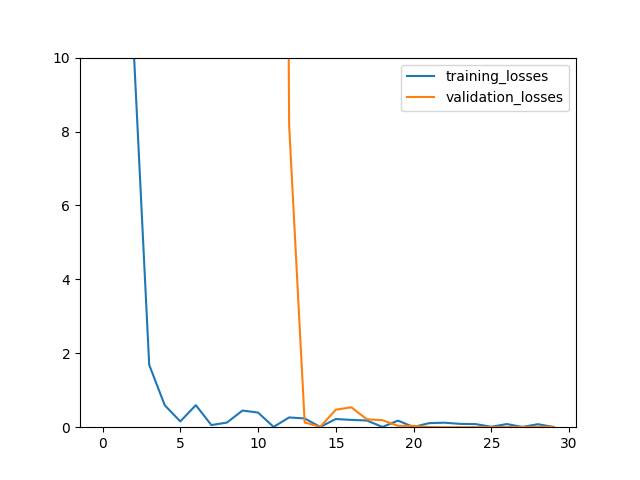
\includegraphics[scale=.4]{images/bestplot_1.png}
  \caption{Best parameters for first kind of plot}
\end{figure}
\begin{figure}
  \centering
  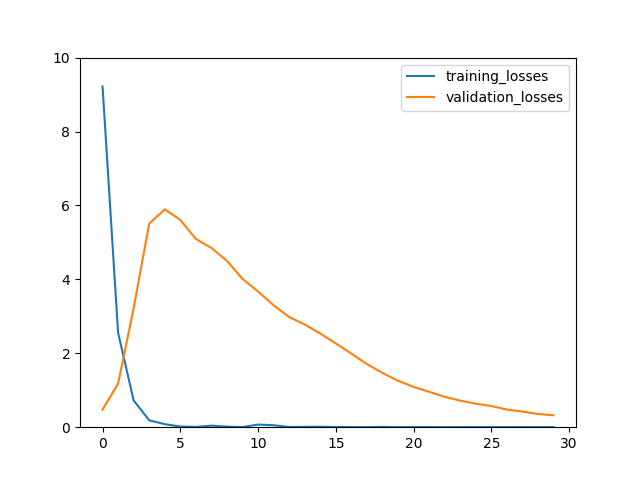
\includegraphics[scale=.4]{images/bestplot_2.png}
  \caption{Best parameters for second kind of plot}
\end{figure}

\section{Conclusion}

\bibliographystyle{IEEEtran}
\bibliography{project2}

\end{document}